\documentclass[a4paper,10pt,twoside]{article}

\usepackage[top=1in, bottom=1in, left=1in, right=1in]{geometry}
\usepackage[utf8]{inputenc}
\usepackage[spanish,es-ucroman,es-noquoting]{babel}
\usepackage{setspace}
\usepackage{fancyhdr}
\usepackage{lastpage}
\usepackage{amsmath}
\usepackage{amsfonts}
\usepackage{verbatim}
\usepackage{float}
\usepackage{graphicx}
\usepackage{subcaption}
\usepackage{amssymb}
\usepackage{url}
\usepackage{moreverb}


% Evita que el documento se estire verticalmente para ocupar
% el espacio vacío en cada página.
\raggedbottom


%%%%%%%%%% Configuración de Fancyhdr - Inicio %%%%%%%%%%
\pagestyle{fancy}
\thispagestyle{fancy}
\lhead{Trabajo Práctico 2, Organización del Computador II}
\rhead{Capra, Lovisolo, Petaccio}
\renewcommand{\footrulewidth}{0.4pt}
\cfoot{\thepage /\pageref{LastPage}}

\fancypagestyle{caratula} {
   \fancyhf{}
   \cfoot{\thepage /\pageref{LastPage}}
   \renewcommand{\headrulewidth}{0pt}
   \renewcommand{\footrulewidth}{0pt}
}
%%%%%%%%%% Configuración de Fancyhdr - Fin %%%%%%%%%%


\begin{document}


%%%%%%%%%%%%%%%%%%%%%%%%%%%%%%%%%%%%%%%%%%%%%%%%%%%%%%%%%%%%%%%%%%%%%%%%%%%%%%%
%% Carátula                                                                  %%
%%%%%%%%%%%%%%%%%%%%%%%%%%%%%%%%%%%%%%%%%%%%%%%%%%%%%%%%%%%%%%%%%%%%%%%%%%%%%%%


\thispagestyle{caratula}

\begin{center}


\includegraphics[height=2cm]{DC.png} 
\hfill

\includegraphics[height=2cm]{UBA.jpg} 

\vspace{2cm}

Departamento de Computación,\\
Facultad de Ciencias Exactas y Naturales,\\
Universidad de Buenos Aires

\vspace{1cm}

\begin{spacing}{2.5}
\begin{Huge}
Reducción de Ruido con la \\Transformada Discreta del Coseno
\end{Huge}
\end{spacing}

\vspace{1cm}

Trabajo Práctico 1, \\
Métodos Numéricos, \\
Primer Cuatrimestre de 2013

\vspace{6cm}

\begin{tabular}{|c|c|c|}
\hline
Apellido y Nombre & LU & E-mail\\
\hline
María Candela Capra Coarasa & 234/11 & canduh\_27@hotmail.com\\
Leandro Lovisolo            & 645/11 & leandro@leandro.me\\
Lautaro José Petaccio       & 443/11 & lausuper@gmail.com\\
\hline
\end{tabular}

\end{center}
\vspace{1cm}

\textbf{Resumen:} \\
Se aplican distintos métodos para agregar ruido a señales sonoras e imágenes para luego, utilizando la Transformada Discreta del Coseno, plantear y sacar conclusiones sobre la eficiencia de varias técnicas de reducción del ruido agregado.

\textbf{Palabras clave:}
DCT, ruido, sonido, imágenes, PSNR, frecuencia.

\newpage


%%%%%%%%%%%%%%%%%%%%%%%%%%%%%%%%%%%%%%%%%%%%%%%%%%%%%%%%%%%%%%%%%%%%%%%%%%%%%%%
%% Índice                                                                    %%
%%%%%%%%%%%%%%%%%%%%%%%%%%%%%%%%%%%%%%%%%%%%%%%%%%%%%%%%%%%%%%%%%%%%%%%%%%%%%%%


\tableofcontents

\newpage


%%%%%%%%%%%%%%%%%%%%%%%%%%%%%%%%%%%%%%%%%%%%%%%%%%%%%%%%%%%%%%%%%%%%%%%%%%%%%%%
%% Introducción Teórica                                                      %%
%%%%%%%%%%%%%%%%%%%%%%%%%%%%%%%%%%%%%%%%%%%%%%%%%%%%%%%%%%%%%%%%%%%%%%%%%%%%%%%


\section{Introducción Teórica}

En este trabajo exploramos un conjunto de métodos basados en la Transformada Discreta del Coseno para eliminar ruidos aperiódicos sobre muestras de señales de una y dos dimensiones (ejemplo: audio e imágenes, respectivamente).

La Transformada Discreta del Coseno, de ahora en más DCT, permite expresar un vector en $\mathbb{R}^n$ como combinación lineal de vectores de la forma $\{(cos(0 * t_0), \ldots cos(0 * t_{n-1})), \ldots (cos(n-1 * t_0), \ldots cos(n-1 * t_{n-1})) \}$, donde n es el tamaño de la muestra y $t_i = (i + \frac{1}{2})\frac{\pi}{n}$. Gráficamente, se puede interpretar este cambio de base como la escritura de la muestra como una suma de cosenos de distintas frecuencias, donde las coordenadas del vector transformado son coeficientes que determinan la amplitud de cada coseno, y se presentan ordenados de menor a mayor frecuencia.

En el caso de señales bidimensionales representadas con matrices $\mathbb{R}^{n \times n}$, la matriz transformada obtenida es análoga al caso unidimensional, en la que se pueden obtener los coeficientes ordenados de menor a mayor frecuencia recorriendo las coordenadas diagonalmente de derecha a izquierda y arriba a abajo, partiendo de la coordenada superior izquierda.


%%%%%%%%%%%%%%%%%%%%%%%%%%%%%%%%%%%%%%%%%%%%%%%%%%%%%%%%%%%%%%%%%%%%%%%%%%%%%%%
%% Desarrollo                                                                %%
%%%%%%%%%%%%%%%%%%%%%%%%%%%%%%%%%%%%%%%%%%%%%%%%%%%%%%%%%%%%%%%%%%%%%%%%%%%%%%%


\section{Desarrollo}

\subsection{Métodos de generación de ruido}
Evaluamos dos métodos para reducir los tipos de ruido descritos a continuación. Para cada método realizamos una serie de experimentos con distintos tipos de muestras, y utilizamos la ecuación de \textit{peak signal-noise ratio}, de ahora en más PSNR\footnote{La fórmula del PSNR se encuentra en el apéndice A.} para medir el nivel de información recuperado. 

Los tipos de ruido tratados son los siguientes:

\subsubsection{Ruido aditivo}

Suma a cada elemento de la muestra una variable aleatoria. En nuestros experimentos, utilizamos variables aleatorias con distribución normal, con media cero y varianza 10.

Observamos que estos parámetros generan una deformación perceptible en todas nuestras muestras, pero no las distorsionan al punto de volverse irreconocibles.

\subsubsection{Ruido impulsivo:}

Reemplaza cada elemento de la muestra por $max$ o $min$ con probabilidad $p$, donde $max$ y $min$ representan el valor máximo y mínimo que adquieren los elementos de la muestra, y $p$ variable de acuerdo al experimento.

Utilizamos $p = 0.01$ en todos nuestros experimentos. Observamos que probabilidades más altas distorsionan demasiado las muestras y dificultan el análisis.


\subsection{Métodos de eliminación de ruido}

Presentamos los dos métodos evaluados a continuación.

\subsubsection{Umbralar}
Dado un umbral $\beta$ y un índice $i$, anulamos todos los coeficientes con índice mayor o igual a $i$ y valor absoluto menor a $\beta$.

Por los mismos motivos analizados en el método \textit{Atenuar}, usamos índices $i = n * 0.5$ e $i = n * 0.3$ para el caso de muestras unidimensionales y bidimensionales, respectivamente.

Despues de probar con distintos umbrales, logramos maximizar el PSNR obtenido utilizando $\beta = (max - min) * 0.1$ en la mayoría de los experimentos realizados, donde $max$ y $min$ representan el valor máximo y mínimo que adquieren los elementos de la muestra.

\subsubsection{Atenuar}
Dados una constante $k$ y un índice $i$, multiplicamos por $k$ los coeficientes de la señal transformada con índice mayor o igual a $i$.

Decidimos usar índices $i = n * 0.5$ e $i = n * 0.3$ para el caso de muestras unidimensionales y bidimensionales, respectivamente. Para las muestras evaluadas, estos índices maximizan el nivel de PSNR observados luego de aplicar el método. Al transformar estas muestras, observamos que el grueso de la información se encuentra en los coeficientes más bajos, y por lo tanto al atenuar los coeficientes correspondientes a frecuecias más elevadas se produce una mejora en la relación señal ruido dejando intactos los coeficientes con la mayoría de la información.

Similarmente, el $k$ elegido es $0.1$. Valores más altos no logran reducir significativamente el ruido, y anular los coeficientes de índice mayor a $i$ implica una importante pérdida de información.


\section{Resultados}
\subsection{Interpretación de resultados}
\begin{itemize}
\item Las figuras correspondientes a la DCT de las imágenes (figuras 6, 10, 16 y 20) fueron creados recorriendo las matrices transformadas de las imágenes en forma diagonal de abajo hacia arriba.

Las figuras figuras 2, 4, 8, 12, 14 y 18 corresponden a la DCT de las señales.

Estas imágenes tienen como intención mostrar como el ruido modifica la DCT y como actúa el método de eliminación de ruido.
\item En cada resultado se identifica el PSNR resultante del ruido agregado y el PSNR final relacionado a la perturbación restante después de aplicar el método de eliminación del ruido.
\end{itemize}

%%%%%%%%%%%%%%%%%%%%%%%%%%%%%%%%%%%%%%%%%%%%%%%%%%%%%%%%%%%%%%%%%%%%%%%%%%%%%%%
%% Atenuar                                                                   %%
%%%%%%%%%%%%%%%%%%%%%%%%%%%%%%%%%%%%%%%%%%%%%%%%%%%%%%%%%%%%%%%%%%%%%%%%%%%%%%%

\subsection{Atenuar}

Presentamos a continuación los resultados de distintos experimentos aplicando este método.

\subsubsection{Ruido aditivo en audio}

\begin{description}
  \item[Muestra:] ramp1234.txt
  \item[PSNR ruido agregado:] 22.55 dB
  \item[PSNR final:] 25.03 dB
\end{description}

\begin{figure}[H]
  \centering
  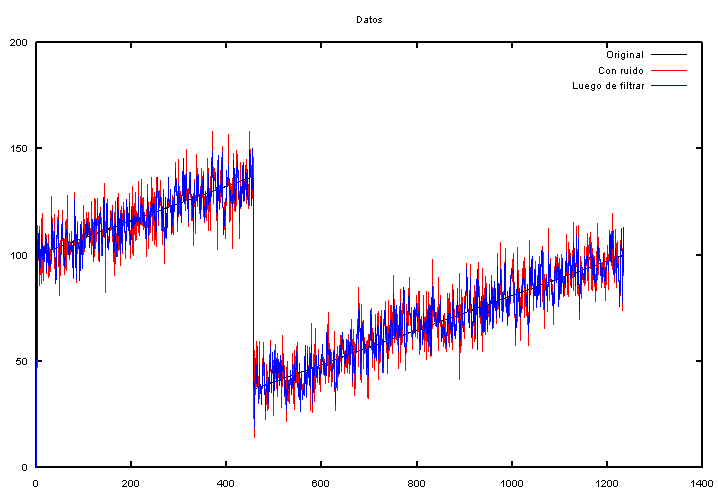
\includegraphics[width=15cm]{graficos/ramp_aditivo_atenuar_muestra.png}
  \caption{Muestra en base canónica.}
\end{figure}

\begin{figure}[H]
  \centering
  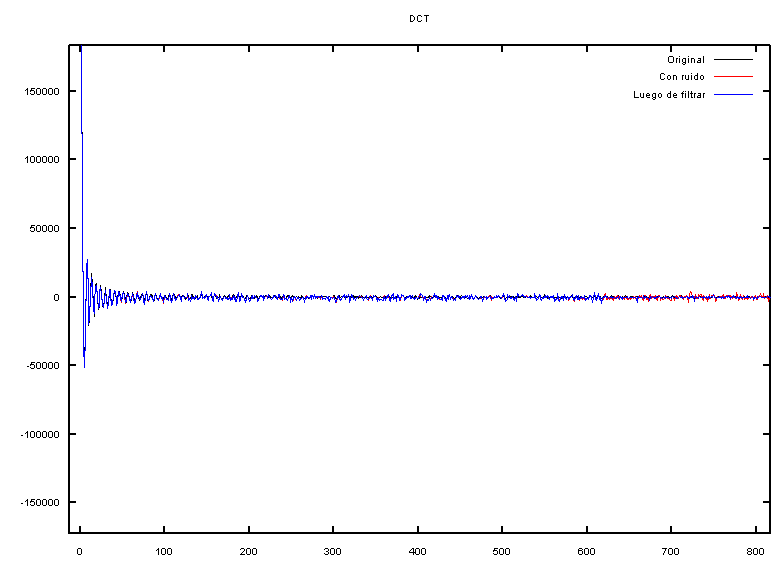
\includegraphics[width=15cm]{graficos/ramp_aditivo_atenuar_dct.png} 
  \caption{Muestra en base DCT.}
\end{figure}


\begin{description}
  \item[Muestra:] dopp512.txt
  \item[PSNR ruido agregado:] 14.02 dB
  \item[PSNR final:] 16.28 dB
\end{description}

\begin{figure}[H]
  \centering
  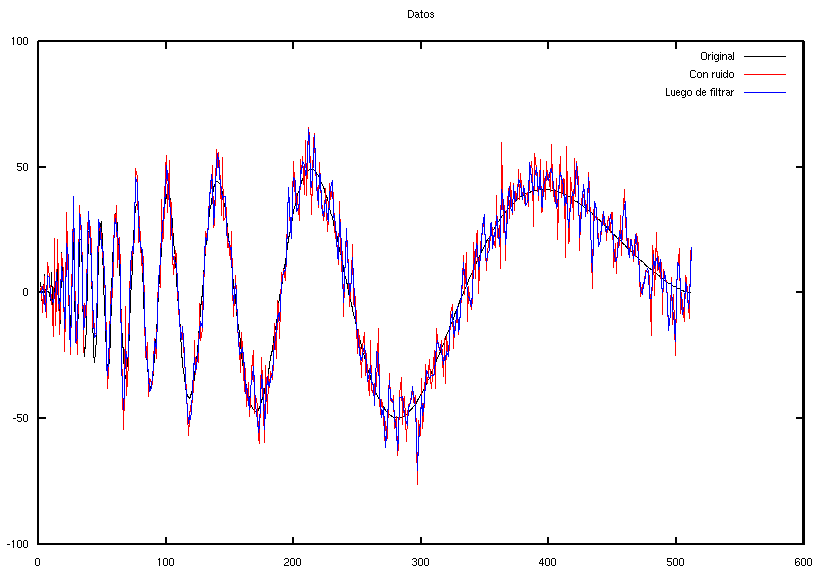
\includegraphics[width=15cm]{graficos/dopp_aditivo_atenuar_muestra.png}
  \caption{Muestra en base canónica.}
\end{figure}

\begin{figure}[H]
  \centering
  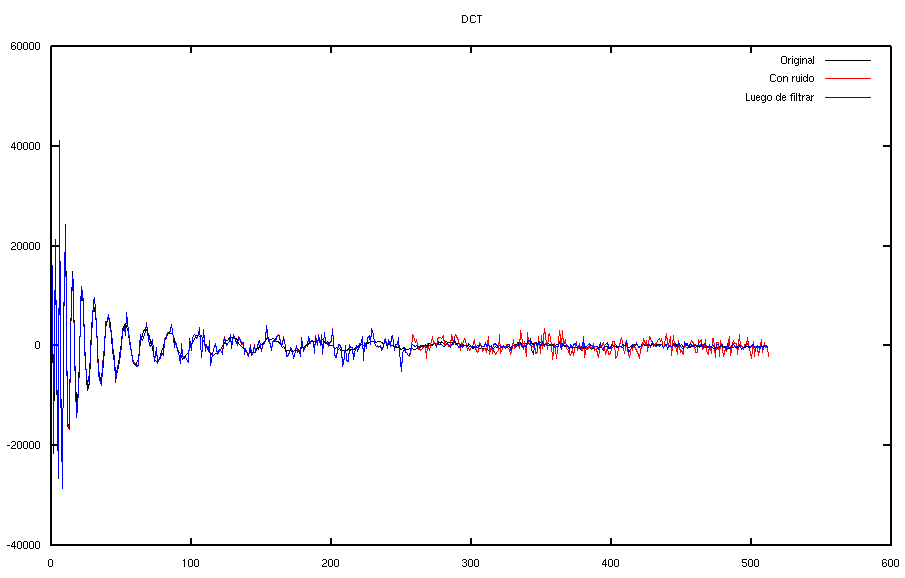
\includegraphics[width=15cm]{graficos/dopp_aditivo_atenuar_dct.png} 
  \caption{Muestra en base DCT.}
\end{figure}


\subsubsection{Ruido aditivo en imágenes}

\begin{description}
  \item[Muestra:] lena.pgm
  \item[PSNR ruido agregado:] 27.23 dB
  \item[PSNR final:] 28.62 dB
\end{description}

\begin{figure}[H]
  \centering
  \begin{subfigure}[b]{0.45\textwidth}
    \centering
    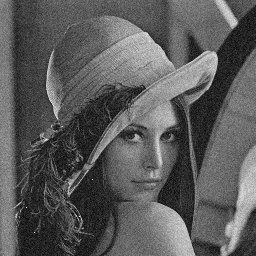
\includegraphics[width=\textwidth]{graficos/lena_aditivo_muestra.png}    
    \caption{Antes de atenuar.}
  \end{subfigure}
  ~ 
  \begin{subfigure}[b]{0.45\textwidth}
    \centering
    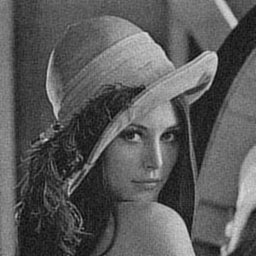
\includegraphics[width=\textwidth]{graficos/lena_aditivo_atenuar_muestra.png}
    \caption{Después de atenuar.}
  \end{subfigure}
  \caption{Ruido aditivo en imágenes.}
\end{figure}

\begin{figure}[H]
  \centering
  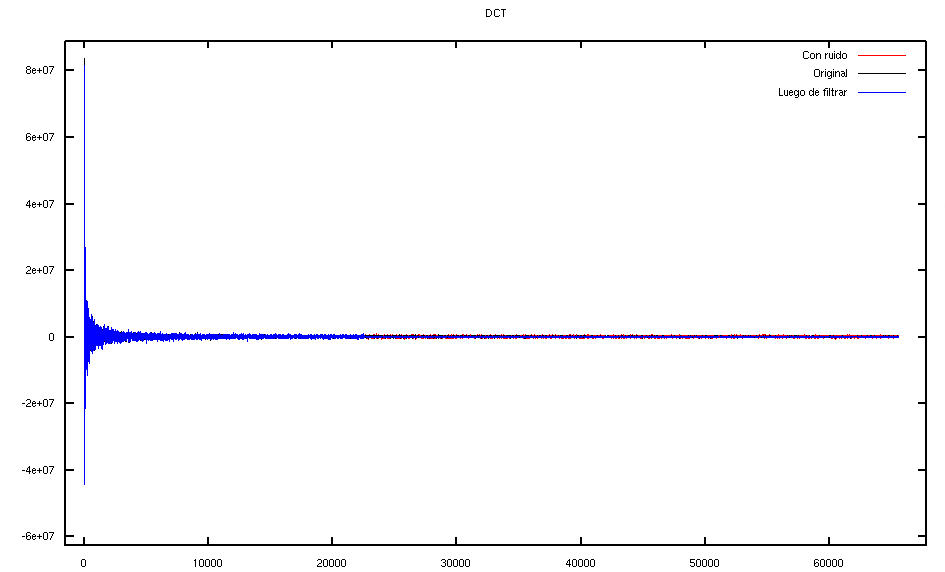
\includegraphics[width=15cm]{graficos/lena_aditivo_atenuar_dct.png} 
  \caption{Muestra en base DCT.}
\end{figure}


\subsubsection{Ruido impulsivo en audio}

\begin{description}
  \item[Muestra:] dopp512.txt
  \item[PSNR ruido agregado:] 15.54 dB
  \item[PSNR final:] 17.55 dB
\end{description}

\begin{figure}[H]
  \centering
  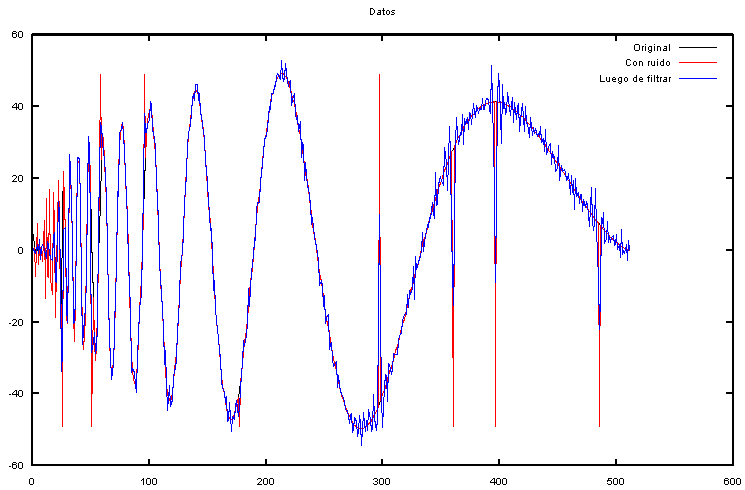
\includegraphics[width=15cm]{graficos/dopp_impulsivo_atenuar_muestra.png} 
  \caption{Muestra en base canónica.}
\end{figure}

\begin{figure}[H]
  \centering
  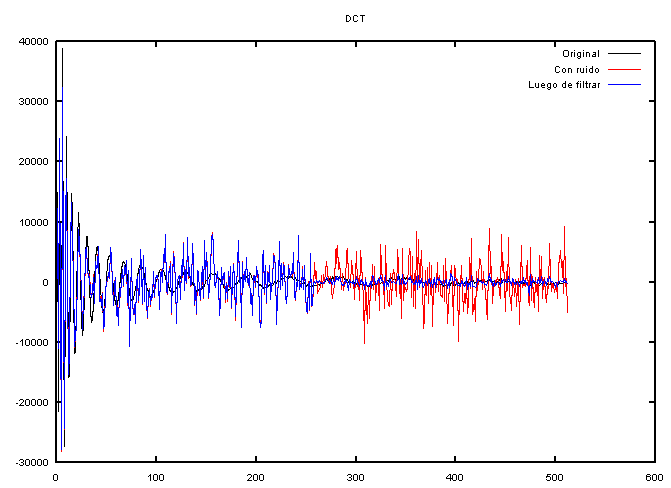
\includegraphics[width=15cm]{graficos/dopp_impulsivo_atenuar_dct.png} 
  \caption{Muestra en base DCT.}
\end{figure}


\subsubsection{Ruido impulsivo en imágenes}

\begin{description}
  \item[Muestra:] lena.pgm
  \item[PSNR ruido agregado:] 21.53 dB
  \item[PSNR final:] 24.92 dB
\end{description}

\begin{figure}[H]
  \centering
  \begin{subfigure}[b]{0.45\textwidth}
    \centering
    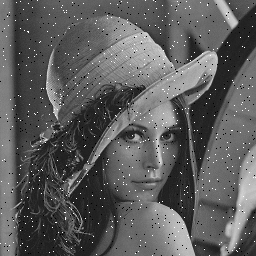
\includegraphics[width=\textwidth]{graficos/lena_impulsivo_muestra.png}    
    \caption{Antes de atenuar.}
  \end{subfigure}
  ~ 
  \begin{subfigure}[b]{0.45\textwidth}
    \centering
    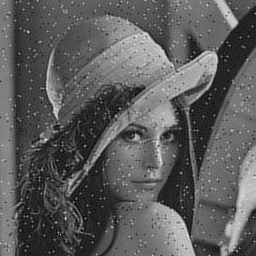
\includegraphics[width=\textwidth]{graficos/lena_impulsivo_atenuar_muestra.png}
    \caption{Después de atenuar.}
  \end{subfigure}
  \caption{Ruido impulsivo en imágenes.}
\end{figure}

\begin{figure}[H]
  \centering
  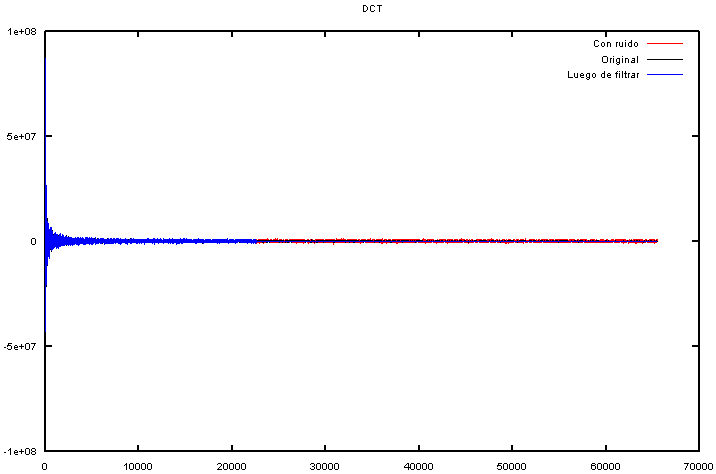
\includegraphics[width=15cm]{graficos/lena_impulsivo_atenuar_dct.png} 
  \caption{Muestra en base DCT.}
\end{figure}


%%%%%%%%%%%%%%%%%%%%%%%%%%%%%%%%%%%%%%%%%%%%%%%%%%%%%%%%%%%%%%%%%%%%%%%%%%%%%%%
%% Umbralar                                                                  %%
%%%%%%%%%%%%%%%%%%%%%%%%%%%%%%%%%%%%%%%%%%%%%%%%%%%%%%%%%%%%%%%%%%%%%%%%%%%%%%%


\subsection{Umbralar}

\subsubsection{Ruido aditivo en audio}

\begin{description}
  \item[Muestra:] ramp1234.txt
  \item[PSNR ruido agregado:] 22.54 dB
  \item[PSNR final:] 24.60 dB
\end{description}

\begin{figure}[H]
  \centering
  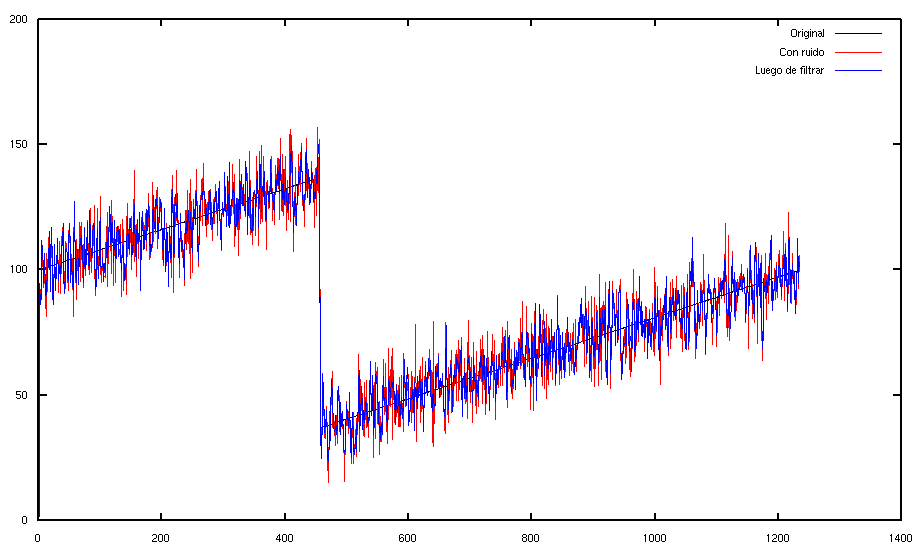
\includegraphics[width=15cm]{graficos/ramp_aditivo_umbralizar_muestra.png}
  \caption{Muestra en base canónica.}
\end{figure}

\begin{figure}[H]
  \centering
  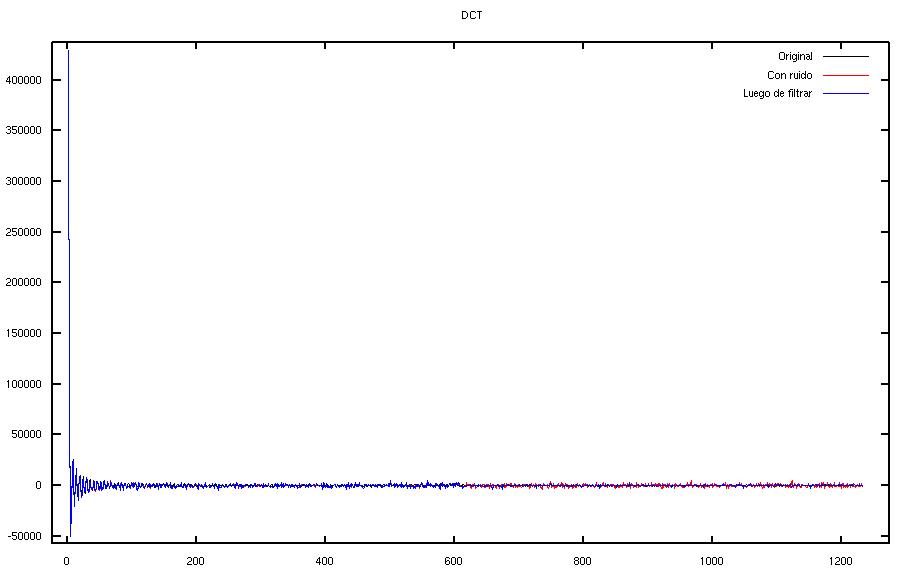
\includegraphics[width=15cm]{graficos/ramp_aditivo_umbralizar_dct.png} 
  \caption{Muestra en base DCT.}
\end{figure}


\begin{description}
  \item[Muestra:] dopp512.txt
  \item[PSNR ruido agregado:] 14.31 dB
  \item[PSNR final:] 16.45 dB
\end{description}

\begin{figure}[H]
  \centering
  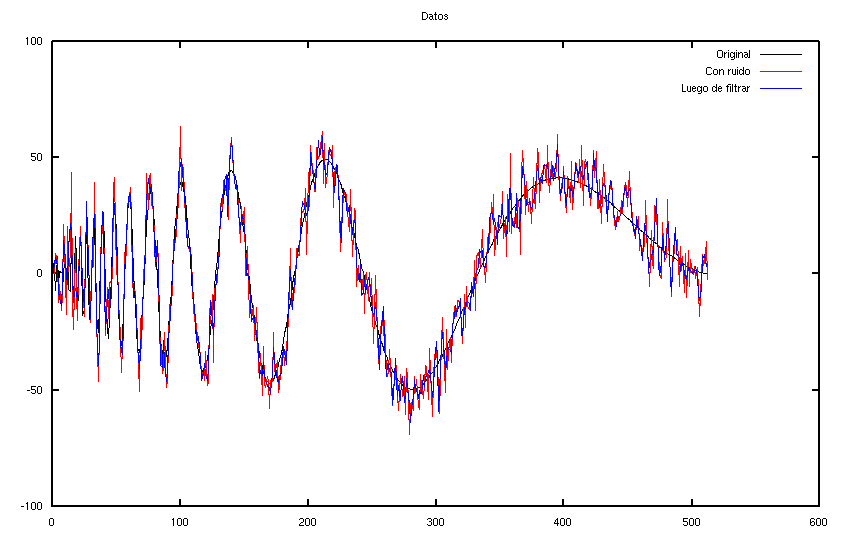
\includegraphics[width=15cm]{graficos/dopp_aditivo_umbralizar_muestra.png}
  \caption{Muestra en base canónica.}
\end{figure}

\begin{figure}[H]
  \centering
  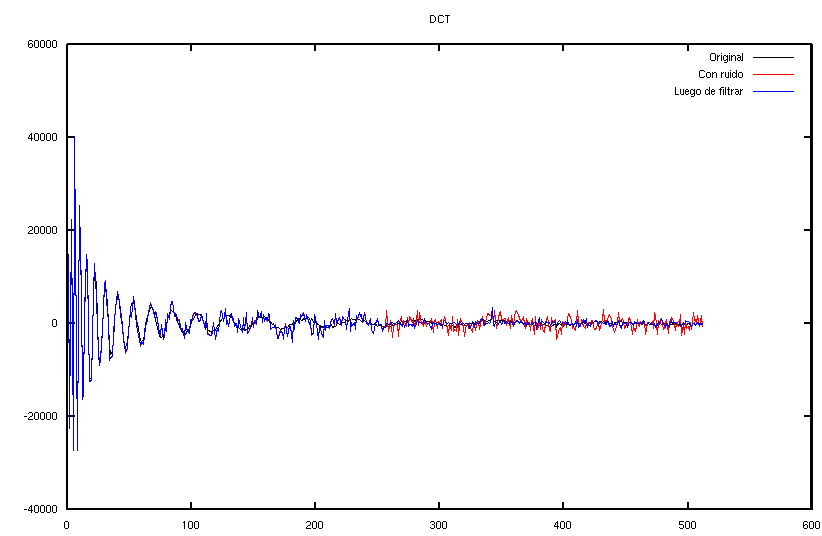
\includegraphics[width=15cm]{graficos/dopp_aditivo_umbralizar_dct.png} 
  \caption{Muestra en base DCT.}
\end{figure}


\subsubsection{Ruido aditivo en imágenes}

\begin{description}
  \item[Muestra:] lena.pgm
  \item[PSNR ruido agregado:] 27.27 dB
  \item[PSNR final:] 28.08 dB
\end{description}

\begin{figure}[H]
  \centering
  \begin{subfigure}[b]{0.45\textwidth}
    \centering
    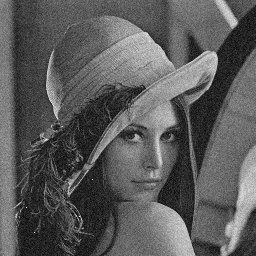
\includegraphics[width=\textwidth]{graficos/lena_aditivo_muestra.png}    
    \caption{Antes de umbralar.}
  \end{subfigure}
  ~ 
  \begin{subfigure}[b]{0.45\textwidth}
    \centering
    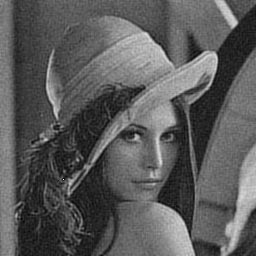
\includegraphics[width=\textwidth]{graficos/lena_aditivo_umbralizar_muestra.png}
    \caption{Después de umbralar.}
  \end{subfigure}
  \caption{Ruido aditivo en imágenes.}
\end{figure}

\begin{figure}[H]
  \centering
  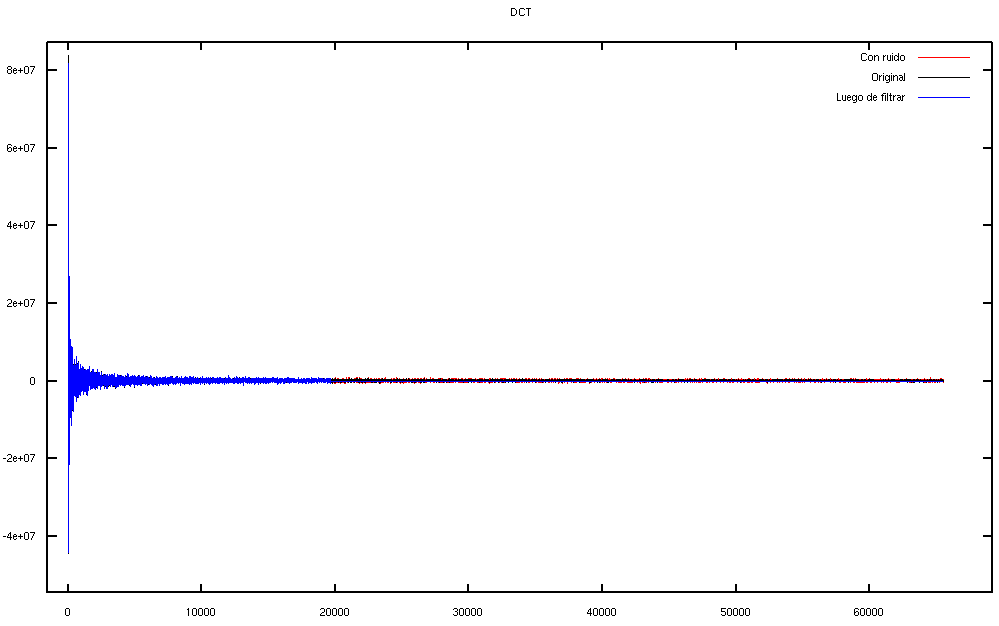
\includegraphics[width=15cm]{graficos/lena_aditivo_umbralizar_dct.png} 
  \caption{Muestra en base DCT.}
\end{figure}


\subsubsection{Ruido impulsivo en audio}

\begin{description}
  \item[Muestra:] dopp512.txt
  \item[PSNR ruido agregado:] 14.87 dB
  \item[PSNR final:] 16.96 dB
\end{description}

\begin{figure}[H]
  \centering
  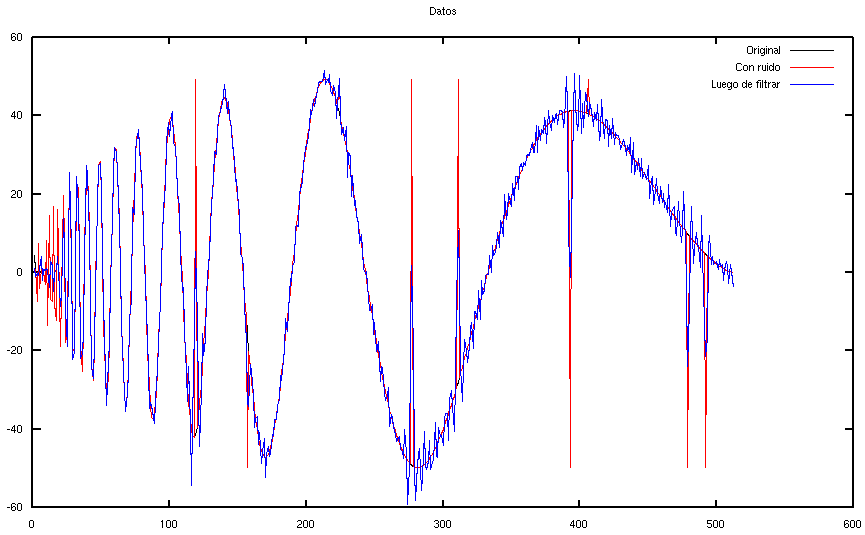
\includegraphics[width=15cm]{graficos/dopp_impulsivo_umbralizar_muestra.png}
  \caption{Muestra en base canónica.}
\end{figure}

\begin{figure}[H]
  \centering
  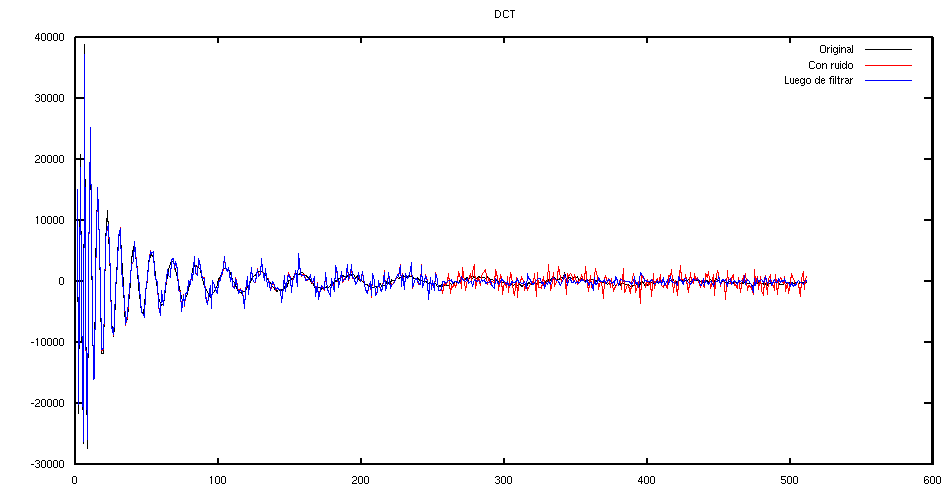
\includegraphics[width=15cm]{graficos/dopp_impulsivo_umbralizar_dct.png} 
  \caption{Muestra en base DCT.}
\end{figure}


\subsubsection{Ruido impulsivo en imágenes}

\begin{description}
  \item[Muestra:] lena.pgm
  \item[PSNR ruido agregado:] 21.39 dB
  \item[PSNR final:] 24.92 dB
\end{description}

\begin{figure}[H]
  \centering
  \begin{subfigure}[b]{0.45\textwidth}
    \centering
    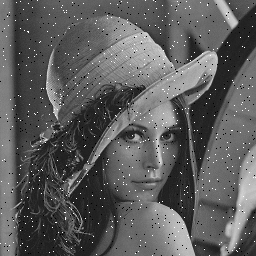
\includegraphics[width=\textwidth]{graficos/lena_impulsivo_muestra.png}    
    \caption{Antes de umbralar.}
  \end{subfigure}
  ~ 
  \begin{subfigure}[b]{0.45\textwidth}
    \centering
    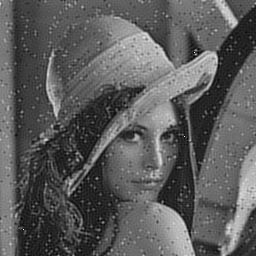
\includegraphics[width=\textwidth]{graficos/lena_impulsivo_umbralizar_muestra.png}
    \caption{Después de umbralar.}
  \end{subfigure}
  \caption{Ruido impulsivo en imágenes.}
\end{figure}

\begin{figure}[H]
  \centering
  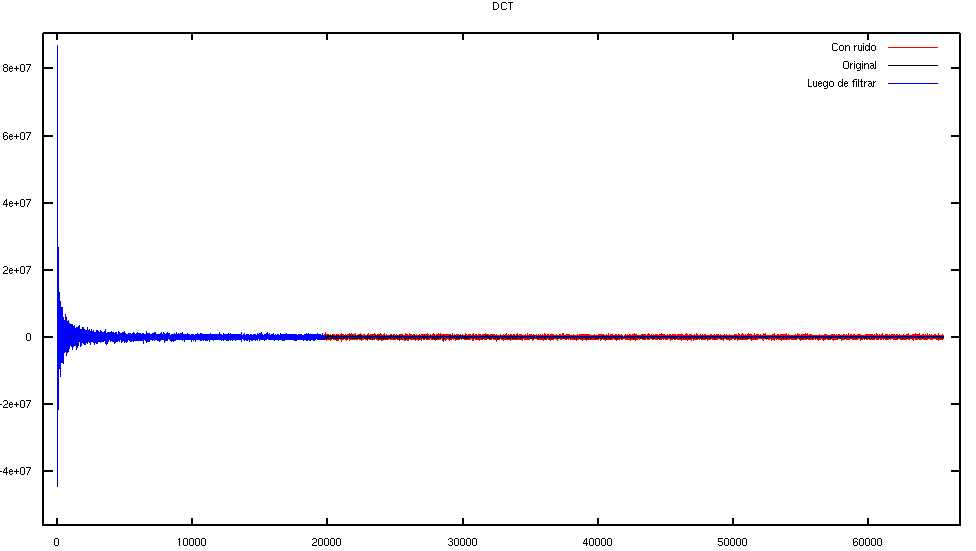
\includegraphics[width=15cm]{graficos/lena_impulsivo_umbralizar_dct.png} 
  \caption{Muestra en base DCT.}
\end{figure}

%%%%%%%%%%%%%%%%%%%%%%%%%%%%%%%%%%%%%%%%%%%%%%%%%%%%%%%%%%%%%%%%%%%%%%%%%%%%%%%
%% Discusión                                                                 %%
%%%%%%%%%%%%%%%%%%%%%%%%%%%%%%%%%%%%%%%%%%%%%%%%%%%%%%%%%%%%%%%%%%%%%%%%%%%%%%%

\section{Discusión}
\subsection{Aplicación sobre ondas}
\subsubsection{Ruido aditivo}
Al observar las figuras relacionadas al ruido aditivo en ondas (figuras 1 y 3 por ejemplo) puede observarse como este tipo de ruido afecta a toda la señal de manera uniforme. La DCT correspondiente a cada figura muestra también estas perturbaciones en todo el rango de frecuencias.
\begin{description}
\item[Método de atenuar sobre ruido aditivo:]
Utilizando el método de atenuar sobre este ruido es posible ver en las imágenes descriptas anteriormente como atenúa el ruido reduciendo los saltos en las ondas que este  produjo aproximandose levemente a la señal original y mostrando un PSNR más bajo.

Puede distinguirse en las figuras de las DCT's correspondientes que la elección del segmento (incluir segmento) y su atenuación produce una interesante atenuación de las perturbaciones creadas por el ruido haciendo que la DCT filtrada sea similar a la DCT sin ruido.
\item[Método de umbralar para ruido aditivo:]
Para el método de umbralar () es posible notar como su aplicación sobre el segmento determinado produce una reducción de la perturbación de la señal, esta reducción se nota menor que en atenuar debido a su naturaleza de "aplanar" (poner en 0) las ondas que superen cierto valor haciendo que en ciertos casos haya una perdida de información.
\end{description}
\subsubsection{Ruido impulsivo}
En el caso del ruido impulsivo en ondas se puede observar (figuras 7 y 17) como este ruido conserva la señal en su estado original exceptuando en ciertos puntos dónde se produce un pico hacia su punto mínimo o máximo.
\begin{description}
\item[Método de atenuar para ruido impulsivo:]
Puede observarse que aplicando atenuar sobre el intervalo determinado se producen alteraciones en otras partes de la señal que no las presentaban antes pero se puede notar que el método logra atenuar en cierta medida los saltos agregados por el ruido.
\item[Método de umbralar para ruido impulsivo:]
\end{description}

\subsection{Aplicación sobre imágenes}
\subsubsection{Ruido aditivo}
\subsubsection{Ruido impulsivo}
%%%%%%%%%%%%%%%%%%%%%%%%%%%%%%%%%%%%%%%%%%%%%%%%%%%%%%%%%%%%%%%%%%%%%%%%%%%%%%%
%% Conclusiones                                                              %%
%%%%%%%%%%%%%%%%%%%%%%%%%%%%%%%%%%%%%%%%%%%%%%%%%%%%%%%%%%%%%%%%%%%%%%%%%%%%%%%


\section{Conclusiones}

En el caso de las imágenes, observamos que al transformarlas al dominio de la DCT, los coeficientes de frecuencias más bajas contienen la mayoría de la información. Observamos además que los ruidos analizados modifican los coeficientes más altos de la imagen, donde se definen los detalles más finos de la misma. Esto nos permite reducir este tipo de ruido fácilmente sin una pérdida signficativa de información reduciendo o eliminando los coeficientes de frecuencias altas.

En contraste, los tipos de ruidos evaluados sobre señales unidimensionales se manifiestan en todos los coeficientes en el espacio de la DCT. No obstante, las muestras evaluadas presentan el grueso de la información en coeficientes medios y bajos, por lo que es posible alcanzar una mejora en PSNR atenuando los coeficientes de frecuencias más elevadas sin pérdidas significativas de información. Esto significa que la muestra resultante conserva el ruido original, pero con menor intensidad en las frecuencias más altas.

En cuanto a los métodos analizados, observamos incrementos de PSNR similares en ambos métodos, pero \textit{Atenuar} resulta superior a \textit{Umbralar} en casi todos los experimentos, ya que conserva más información al atenuar coeficientes en lugar de eliminarlos completamente. 

En conclusión, los métodos basados en la DCT resultan una buena herramienta para eliminar estos tipos de ruido presentes en imágenes. Al aplicarlos en señales unidimensionales también se obtiene una mejora en el PSNR, pero menor que el caso bidimensional ya que no modifican el ruido en sus coeficientes más bajos.


%%%%%%%%%%%%%%%%%%%%%%%%%%%%%%%%%%%%%%%%%%%%%%%%%%%%%%%%%%%%%%%%%%%%%%%%%%%%%%%
%% Apéndice A: Enunciado del Trabajo Práctico                                %%
%%%%%%%%%%%%%%%%%%%%%%%%%%%%%%%%%%%%%%%%%%%%%%%%%%%%%%%%%%%%%%%%%%%%%%%%%%%%%%%

\newpage

\section{Apéndice A: Enunciado del Trabajo Práctico}

\parskip = 10pt

\newcommand{\real}{\mathbb{R}}

{\bf Introducci\'on}

La Transformada Discreta del Coseno  (DCT, por sus siglas en ingl\'es) es una herramienta que nos permite representar cualquier se\~nal en el plano de las frecuencias. Dado que es utilizada por el est\'andar de compresi\'on de im\'agenes JPEG y formato de video MPEG, se encuentra implementada en m\'as lugares de lo que pensamos: en cada c\'amara digital o tel\'efono m\'ovil. 
La DCT no solo tiene aplicaciones al mundo de la compresi\'on (donde los valores transformados pueden ser codificados de forma eficiente), sino tambi\'en al procesamiento: el an\'alisis de qu\'e frecuencias est\'an presentes en las se\~nales es esencial en ciertos contextos de aplicaci\'on.

La idea intuitiva de esta transformada, en el plano continuo, consiste en representar una funci\'on $f: \mathbb{R} \rightarrow \mathbb{R}$ en la base de funciones $\mathcal{B}=\{1, \cos(x), \cos(2x),...\}$.
En el plano discreto, la DCT se corresponde a un cambio de base: cada una de las funciones de la base $\mathcal{B}$ se discretiza en ciertos puntos pasando a ser una base de vectores en $\mathbb{R}^n$, (donde $n$ es la dimensi\'on del vector o se\~nal a transformar).
Es decir, dado un vector o se\~nal $x\in\mathbb{R}^n$ existe una matriz $M\in\mathbb{R}^{n\times n}$ de cambio de base que define la transformada DCT, donde $y=Mx$ es el vector o se\~nal transformado al espacio de frecuencias por la DCT (ver ap\'endice \ref{sec:dct}). Esta operaci\'on es f\'acilmente extensible a se\~nales de dos dimensiones (ver ap\'endice \ref{sec:dct2d}).


{\bf Enunciado}

El objetivo del trabajo es eliminar ruido sobre una se\~nal ruidosa $x\in\real^{n}$. Para ello se realiza el siguiente proceso: 
\begin{enumerate}
\item  $y:=Mx$ [Transformar usando Ec.~(\ref{eq:dctint}) de Ap. \ref{sec:dct}]
\item $\tilde{y} := f(y)$ [Modificar]
\item Resolver $M \tilde{x} = \tilde{y}$ [Reconstruir]
\end{enumerate}

 
Una forma de medir la calidad visual de la se\~nal reconstruida $\tilde{x}$, es a trav\'es del PSNR ({\em Peak Signal-to-Noise Ratio}).
EL PSNR es una m\'etrica `perceptual' (acorde a lo que perciben los humanos) y nos da una forma de medir la calidad de una imagen perturbada, siempre y cuando se cuente con la se\~nal original. 
Cuanto mayor es el PSNR, mayor es la calidad de la imagen. La unidad de medida es el decibel (db) y se considera que una diferencia de 0.5 db ya es notada por la vista humana. El PSNR se define como:
$$
\mathit{PSNR} = 10 \cdot \log_{10} \left( \frac{\mathit{MAX}^2_x}{\mathit{ECM}} \right)
$$
donde $\mathit{MAX}_x$ define el rango m\'aximo de la se\~nal (en caso de entradas de 8 bits sin signo, ser\'ia 255) y \emph{ECM} es el {\em error cuadr\'atico medio}, definido como:
$ \frac{1}{n} \sum_{i}{(x_{i} - \tilde{x}_{i})^2} $,
donde $n$ es la cantidad de elementos de la se\~nal, $x$ es la se\~nal original y $\tilde{x}$ es la se\~nal recuperada.

En la implementaci\'on realizada deben llevar a cabo los siguientes experimentos:
\begin{itemize}
\item Para varias se\~nales con distintos niveles de ruido, se deber\'an experimentar con al menos 2 estrategias (definiendo $f$ de forma conveniente) para modificar la se\~nal transformada $y$ (paso 2) con el objetivo de que la se\~nal recuperada $\tilde{x}$ contenga menos ruido; se deber\'an extraer conclusiones en cuanto a la calidad de la se\~nal recuperada, en funci\'on de la estrategia utilizada.
\item Se deber\'an repetir los anteriores experimentos tambi\'en sobre im\'agenes adaptando el m\'etodo para aplicar la transformada DCT en dos dimensiones seg\'un se explica en la ap\'endice \ref{sec:dct2d}. 
\item {\bf (Opcional)} Se deber\'a analizar la aplicaci\'on de la DCT `por bloques' sobre im\'agenes. Por ejemplo, si tenemos una imagen de $64\times 64$ p\'ixeles podemos subdividirla en: 4 bloques de $32\times 32$, o 16 bloques de $16\times 16$, o 64 bloques de $8\times 8$, y aplicar la DCT en 2D sobre cada uno de los bloques (considerar un tama\~no m\'inimo de $8\times 8$ para cada bloque).\\ 
Elegir una estrategia utilizada para se\~nales unidimiensionales y sacar conclusiones respondiendo a los siguientes interrogantes (realizando experimentos que justifiquen la respuesta): ?`Es lo mismo eliminar ruido sobre la imagen entera que de a bloques? ?`Qu\'e forma es m\'as conveniente en cuanto a la calidad visual? ?`Qu\'e forma es m\'as r\'apida? 
\end{itemize}

{\bf Formatos de archivos de entrada}

Las se\~nales ser\'an le\'idas de un archivo de texto en cuya primer l\'inea figuran la cantidad de datos y en la l\'inea siguiente se encuentran los datos en ASCII separados por espacios. Para leer y escribir im\'agenes sugerimos utilizar el formato {\em raw} binario \texttt{.pgm}\footnote{\url{http://netpbm.sourceforge.net/doc/pgm.html}}. 
El mismo es muy sencillo de implementar y compatible con muchos gestores de fotos\footnote{XnView \url{http://www.xnview.com/}} y Matlab.

\vskip 0.5 cm
\hrule
\vskip 0.1 cm

{\bf Fecha de entrega:} 
\begin{itemize}
\item \textsl{Formato electr\'onico:} jueves 16 de mayo de 2013, hasta las 23:59 hs., enviando el trabajo (informe+c\'odigo) a \texttt{metnum.lab@gmail.com}. El subject del email debe comenzar con el texto \verb|[TP2]| seguido de la lista de apellidos de los integrantes del grupo. 
\item \textsl{Formato f\'isico:} viernes 17 de abril de 2013, de 18 a 20hs (en la clase del labo).
\end{itemize}

\subsection{Transformada Coseno Discreta}\label{sec:dct}

Para generar la matriz $M\in\real^{n\times n}$ que define la transformada de Coseno Discreta definimos: 
\begin{itemize}
 \item Vector de frecuencias:  $g = \left(\begin{array}{c} 0 \\ 1 \\ \vdots \\ n-1 \end{array} \right)$
 \item Vector de muestreo: $ s= {\displaystyle \frac{\pi}{n} }\left(\begin{array}{c} \frac{1}{2} \\1+\frac{1}{2} \\  \vdots \\ (n-1)+\frac{1}{2} \end{array} \right) $
 \item Constante de normalizaci\'on: $C(k) = \left\{ \begin{array}{lr}\sqrt{\frac{1}{n}} & k=1 \\ \sqrt{\frac{2}{n}} & k > 1 \end{array} \right.$
\end{itemize}

Siendo $T=\cos(g\cdot s^t)$ la matriz resultante de aplicarle el coseno a cada elemento de la matriz $g\cdot s^t$,
finalmente definimos, $\widehat{M}_{i,j} = C(i) \cdot T_{i,j}$

Para obtener una versi\'on entera de la transformaci\'on que define la matriz $M$, la cual ser\'a aplicada a se\~nales (o vectores) enteras en el rango $[0,q]$, definimos:
\begin{equation}
M = \left\lfloor \frac{q \widehat{M} + 1}{2}  \right\rfloor \label{eq:dctint}
\end{equation} 
donde $\left\lfloor\cdot\right\rfloor$ indica la parte entera inferior\footnote{El redondeo de un n\'umero $m$ pude definirse como $\lfloor m + 1/2 \rfloor$. Luego, $M$ se define como el redondeo de $\widehat{M}\cdot(q/2)$.}. (Es decir, escalamos los elementos de la matriz $M$ por $q/2$ y luego redondeamos los valores.)

\subsubsection{Extensi\'on a 2D}\label{sec:dct2d}
Dada una matriz $B\in\real^{n\times n}$, podemos extender f\'acilmente la transformada DCT a se\~nales de dos dimensiones. Para ello, aplicamos la transformaci\'on por filas y por columnas: $ M\, B\, M^t $




%%%%%%%%%%%%%%%%%%%%%%%%%%%%%%%%%%%%%%%%%%%%%%%%%%%%%%%%%%%%%%%%%%%%%%%%%%%%%%%
%% Apéndice B: Código Fuente                                                 %%
%%%%%%%%%%%%%%%%%%%%%%%%%%%%%%%%%%%%%%%%%%%%%%%%%%%%%%%%%%%%%%%%%%%%%%%%%%%%%%%

\newpage

\section{Apéndice B: Código Fuente}

\subsection{Metodos.cpp}

\verbatimtabinput{../Metodos.cpp}

\subsection{Ecuaciones.cpp}

\verbatimtabinput{../Ecuaciones.cpp}

\subsection{Matriz.h}

\verbatimtabinput{../Matriz.h}

\subsection{Matriz.cpp}

\verbatimtabinput{../Matriz.cpp}


\end{document}